\newpage 
% \setcounter{page}{1} % only for draft purpose to keep page count on track
\section{Forward Plan}

As of writing this there has been a single publication from this project (outlined in \cref{sec:method-technosignature-searches}) with numerous other in preparation for publication. \Cref{fig:gannt_chart} outlines the estimated timeline for the completion of all outlined projects. A brief overview of the projects at their status is outline below in order of expected completion date. 

\begin{figure}[h]
    \centering
    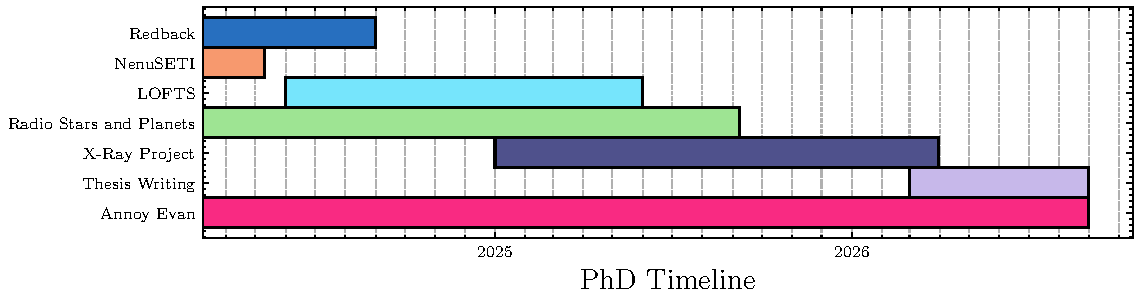
\includegraphics[width=0.95\textwidth]{figs/PhD_gannt_chart.pdf}
    \caption{Estimated timeline for completion of projects that will make up overall PhD. Each increment on the grid is equivalent to 1 month. With the start time marked as March 8th 2024.}
    \label{fig:gannt_chart}
\end{figure}

\subsection{NenuSETI}
This project utilized the New Extension Upgrading LOFAR (NenuFAR) based in Nançay. NenuFAR is the most sensitive standalone low-frequency telescope in the Northern Hemisphere, operating at 10 - 95 MHz. Over the past number of observation cycles, a significant number of observations have been taken. These observations have targeted exoplanets confirmed by Kepler and more recently TESS. Baseband data will be collected for a subset of the TESS catalog in the low frequency band (clean of RFI), reduced into high time and frequency resolution Stokes-I data products at 1.49 Hz and 671 ms resolution, and then finally searched for drifting narrowband signals. As SETI is a key program on NenuFAR, it directly aims to assist other science cases in radio astronomy. \ 

Axis 1: A dedicated TESS exoplanet and targets of interest (TOI) follow-up program, where baseband data will be collected for a subset of the TESS catalog in the 39.8-67.7 MHz band (clean of RFI), reduced into high time and frequency resolution Stokes-I data products at 1.49 Hz and 671 ms resolution, and then finally searched for drifting narrowband signals.

Axis 2: Commensal search associated with the “Exoplanets \& Stars” and “Cosmic Dawn” Key Programs, searching high-resolution data products (of the order of 1 Hz resolution) for artificial emissions originating from distant stellar systems and the Northern Celestial Pole. Moreover, this project will also periodically conduct a high-resolution survey of the RFI environment of NenuFAR and develop an interface for RFI data visualization and analysis. \

The first axis of the NenuSETI project has had 80\% of the analysis completed. This paper is currently being drafted and once some system administration with the BL back-end in Nançay is complete, the paper will be swiftly submitted no later than the end of April 2024. Preliminary constraints set on technosignatures in this frequency range can be seen in \cref{fig:NenuSETI-Parameter-Space}. 

\begin{figure}[h]
    \centering
    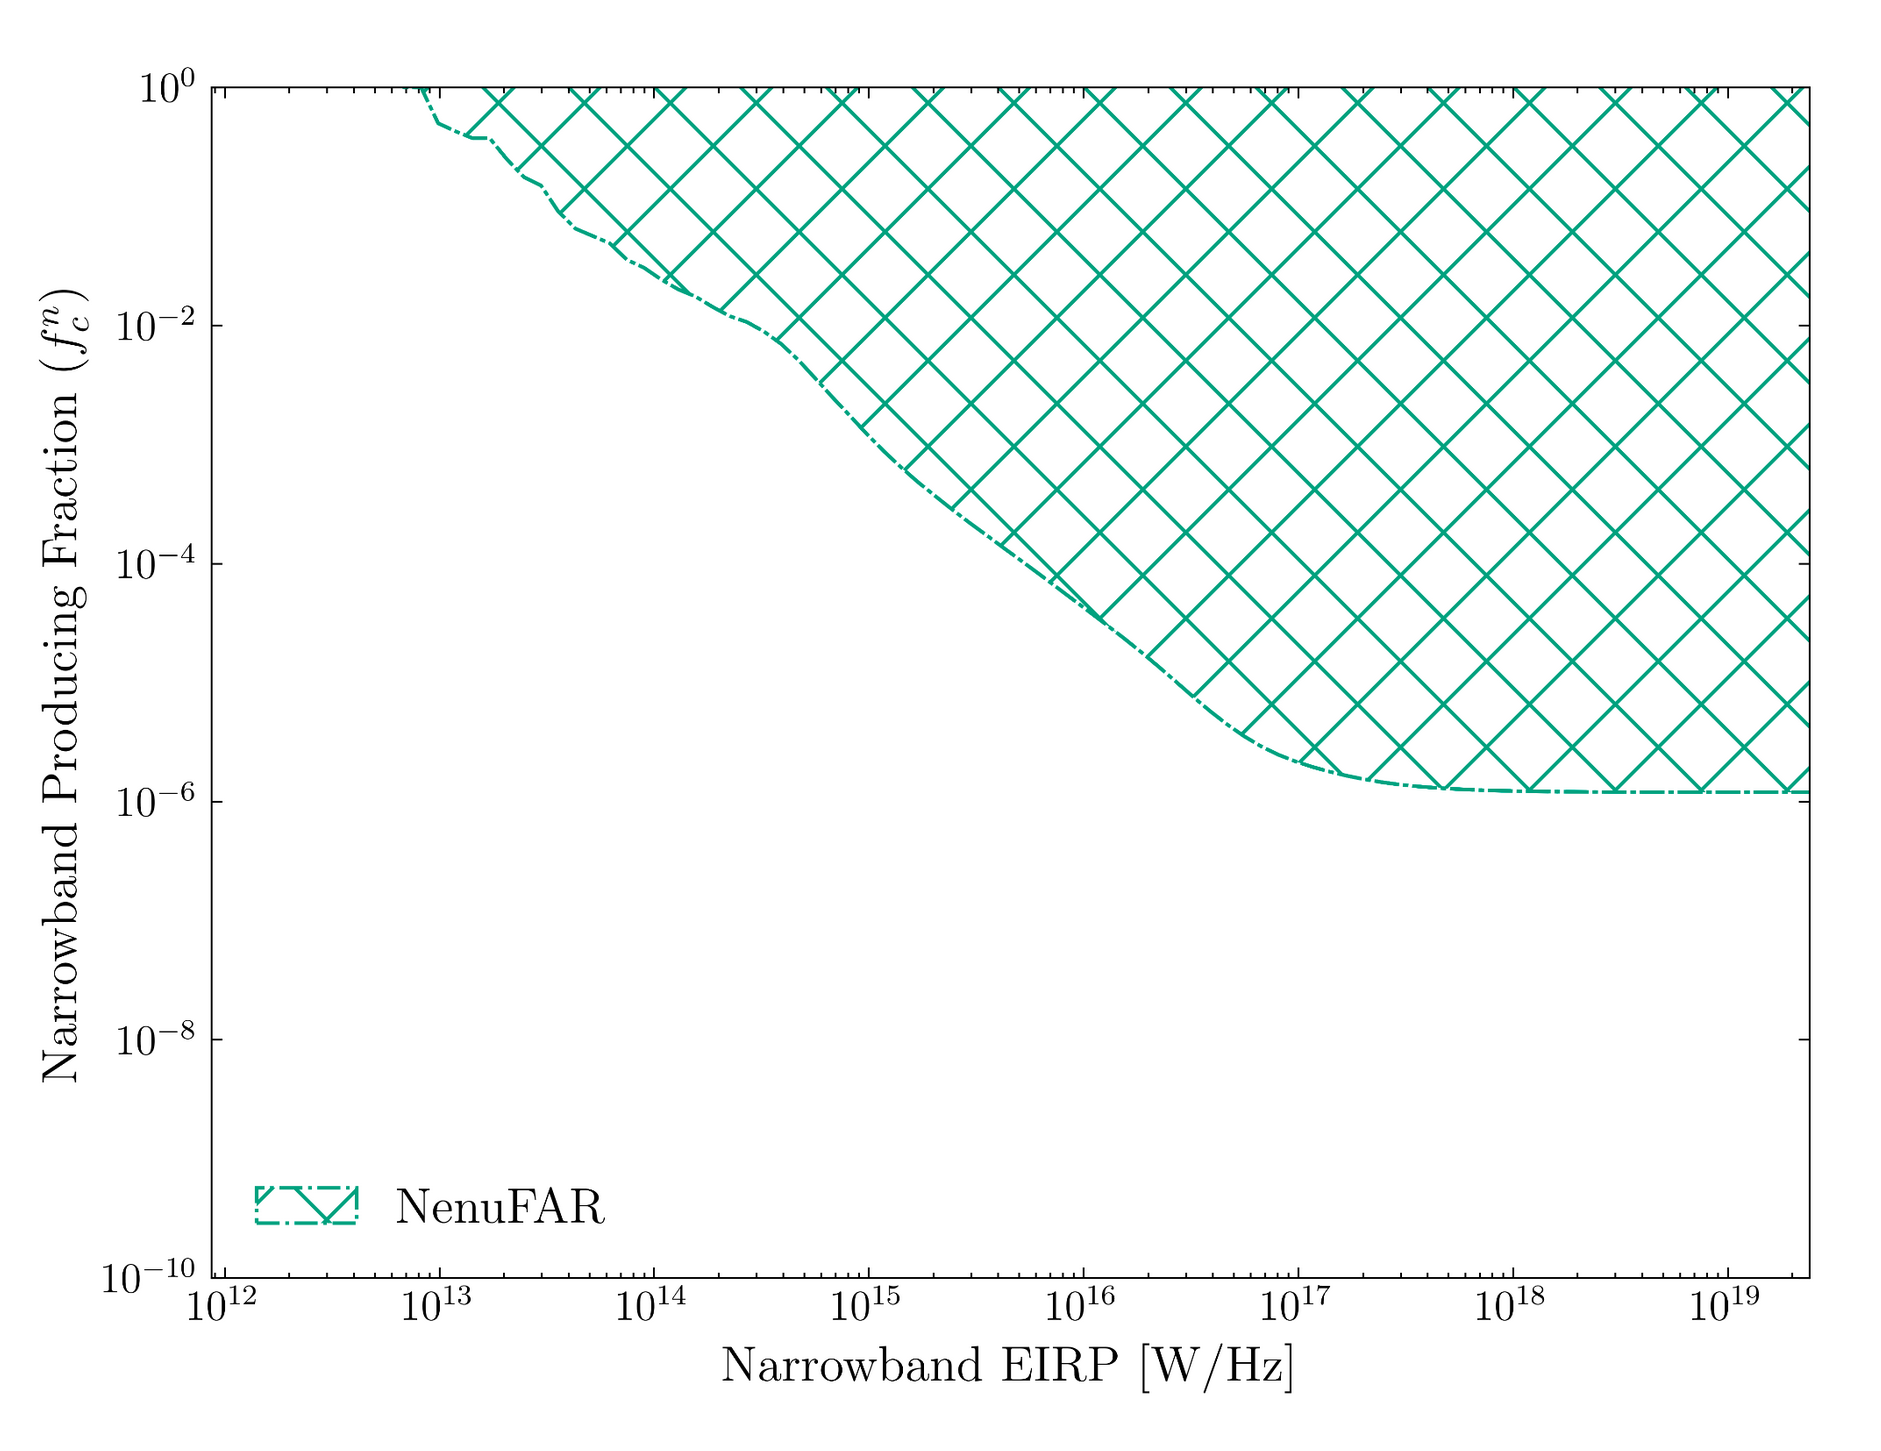
\includegraphics[width = 0.7\textwidth]{figs/NenuFAR-Constraining-Factor.png}
    \caption{The preliminary fraction of stars that produce narrow-band emission ($f^n_c$) against the transmitter power of the total target pool. The hashed region (red) shows the constraints this survey places on a value of $f^n_c$ at 30 - 95 MHz.}
    \label{fig:NenuSETI-Parameter-Space}
\end{figure}

\subsection{Redback Pulsar Searches}
The redback pulsar search employs full analysis pipelines, as detailed in \cref{sec:method-pulsar-searching}, which are written and deployed on the OzStar supercomputing cluster at Swinburne University and the REALTA back-end in Birr. At present, all data from J2059 has been processed, with expanded trials underway in an attempt to detect the pulsar. Processing of data from J2054 is currently at 50\% completion but has been temporarily halted due to bottlenecks in the back-end system. We anticipate publishing either a pulsar detection or non-detection by the end of August 2024. \

\subsection{Low-Frequency FRB, Pulsar and Technosignature Search}

 As previously discussed in \cref{sec:method-technosignature-searches}, the observation campaign is expected to commence following the roll-out of LOFAR 2.0 upgrades to the core stations in the Netherlands. This is anticipated to occur in the early summer months of 2024. Consequently, all remote stations will be allocated 100\% of observing time, allowing for the accommodation of the large amount of observation time required for LOFTS. \ 

Automated pipelines for handling the data have been written and tested on operational backends. The deployment of the BL backend to the Chilboltan station is expected to be completed in the coming months, upgrading the survey's status to tri-site. Methods will be carried out in a similar manner as described in \cref{sec:method-technosignature-searches}.


\subsection{Radio Stars and Exoplanets}

To date, the project has conducted 13 hours of bright M-dwarf observations on two radio bright sources: CR Draconis and TVLM 513-46. The primary objective is to establish a pipeline capable of reliably identifying radio emissions from these sources. Following this, the focus will shift to observing fainter sources, specifically brown dwarfs and planetary systems exhibiting signs of emission resulting from exoplanetary-stellar interactions. \

Observations are taking place on a weekly basis of bright M dwarfs and being actively processed into 8 bit filterbanks in each of the Stoke parameters and searched for evidence of extra solar CMEs. 

% \begin{figure}[h]
%     \centering
%     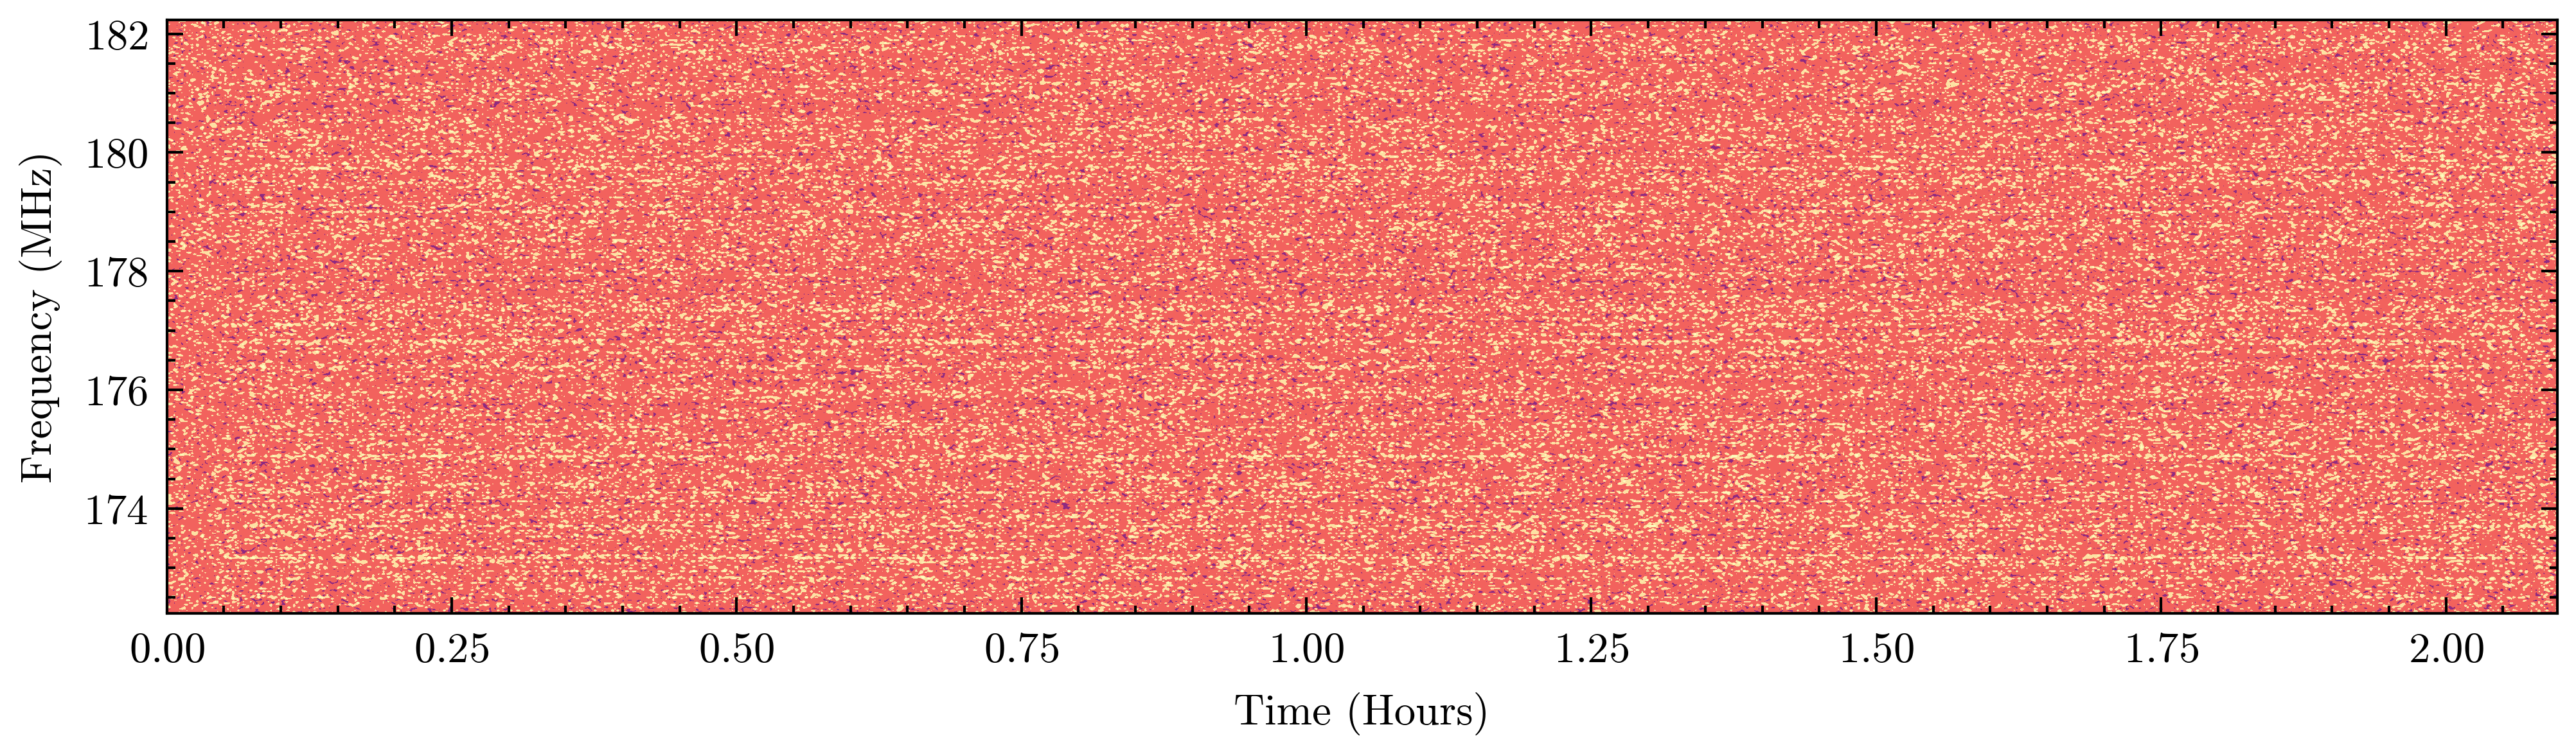
\includegraphics[width = 0.8\textwidth]{figs/CR_Draconis_dynamic_spectra.png}
%     \caption{Dynamic spectra of the non-detection from CR Dra taken from I-LOFAR observation in Stokes I.}
%     \label{fig:CRD_spec}
% \end{figure}

\subsection{Determining the Age of Nearby Young Neutron Stars}
The final project of the thesis aims to determine the age of young nearby Neutron Stars (NS) using archival data from X-ray observatories such as \textit{Chandra} and \textit{XMM Newton}. Young NS have temperatures on the order of $10^6~\text{K}$, which cool quite rapidly within the first $10^{6}~\text{yrs}$. By measuring the blackbody emission from a neutron star,  cooling rate can be determined, thus enabling the estimation of its age. At higher frequencies, observations are essentially blind to DM, making them indistinguishable at even appreciable differences (i.e., 0 -- 40 pc/cc). By pairing measurements with LOFAR, which can determine DM on the scale of $10^{-3}~\text{pc/cc}$. Models of pulsar evolution can be tested once accurate measurements for $P$, $\dot P$, and age have been obtained. 

\newpage
\section{Conclusion}

This report outlines several projects, in \cref{sec:prelude} and \cref{sec:method-pulsar-searching} the theory of redback pulsars and how to search for them were discussed respectively. Unique for their close binary systems, low mass companion and transitional stages they provide a good tool for probing physical parameters of neutron stars. Observations of two \textit{Fermi} redback candidates J0523 and J2054 have been carried out with Parkes and LOFAR respectively. A pipeline has been developed and employed on back-ends connected to each telescope and has successfully detected known pulsars. Further exploration of flag candidates is on going to determine a detection or non-detection of each candidate as described in \cref{sec:folding}. \ 

Additionally, the report describes the theory and methods of the first low-frequency SETI survey in \cref{sec:SETI-th} and \cref{sec:method-technosignature-searches}. The survey encompasses target selection and the search for technosignatures among 1,631,152 targets, providing tight constraints on their prevalence in the Milky Way. The sensitivity to targets across their observed band and their emergence rate are illustrated in \cref{fig:EIRP-limits} and \cref{fig:SETI-constraint}, respectively. Furthermore, outlines for a similar survey with NenuFAR observing \textit{Kepler} and \textit{TESS} targets are discussed, along with plans for a year-long Northern Hemispheric survey with LOFAR to search for both natural and unnatural transients using three stations.

Brief mention is made of ongoing work to explore the feasibility of detecting radio stars and exoplanets using a single LOFAR station. The motivation behind detecting radio emissions from these sources is discussed, along with plans to expand these observations in the coming months. Reliable detection of these sources and application to archival data could reveal new radio-loud M-dwarfs and potentially enable longer observations to detect emissions from ultra-cool dwarfs.

Finally, the last project of the PhD is outlined as an X-Ray project aiming to determine the ages of young neutron stars to better constrain models of neutron star evolution, a challenging and pressing question in the community. Full exploration of both the theory and methodology of this project will be undertaken upon completion of the three aforementioned projects.

